\chapter{The wave function}

\section{The schr\"odinger equation}
Particle's wave function $\Psi(x,t)$ follows the Schr\"odinger equation
\begin{equation}
  \label{eq:1-1}
 i\hbar \frac{\Psi}{\partial t} = - \frac{\hbar^{2}}{2m} \frac{\partial^{2}\Psi}{\partial x^{2}} + V\Psi
\end{equation}
with
\begin{equation}
  \label{eq:1-2}
  \hbar = \frac{h}{2\pi} = 1.054572 \times 10^{-34}Js
\end{equation}

\section{The statistical interpretation}
Born's statistical interpretation of the wave function, which say that $\abs{\Psi\left(x,t\right)}^{2}$ gives the probability of finding the particle at point $x$ at time $t$.
This means
\begin{equation}
  \label{eq:1-3}
  \int_{a}^{b}\abs{\Psi\left(x,t\right)}^{2} dx = \text{Probability of finding particle between a and b at time t.}
\end{equation}

The statistical interpretation introduces a kind of indeterminacy into quantum mechanics.
All quantum mechanics has to offer is statistical information about the possible result.
Suppose I do measure the position of particle, and I find it to be at the point $C$.
Question: Where was the particle just before I made the measurement?
\begin{itemize}
  \item The \textbf{realist} position: The particle was at $C$.
        This certainly seemms like a sensible response, and it is the one Einstein advocated.
        However, this means quantum mechanics is an imcomplete theory, since particle really was at $C$, and yet quantum mechanics was unable to tell us so.
        This indeterminacy is not a fact of nature, bt a reflection of our ignorance.
        Evidently $\Psi$ is not the whole story, some additional information is needed to provide a complete description of the particle.
  \item The \textbf{orthodox} position: The particle wasn't really anywhere.
        It was the act of measurement that forced the particle to ``take a stand''.
        Observations not only disturb what is to be measured, they produce it.
        This view is associated with Bohr and followers.
\end{itemize}

Experiments have decisively confirmed the orthodox interpretation.
A particle simply does not have a precise position prior to measurement, aany more than the ripples on a pond do; it is the measurement process that insists on one particular number, and thereby in a sense creates the specific result, limited only by the statistical weighting imposed by the wave function.

For a second measurement, immediately after the first, the result must be found at $C$.
Since the first measurement radically alters the wave function, so that it is now sharply peaked about $C$.

\section{Normalization}
Since $\abs{\Psi}^{2}$ is the probability density, then we have
\begin{equation}
  \label{eq:1-4}
  \int_{\infty}^{\infty} \abs{\Psi \left(x,t\right)}^{2}dx = 1
\end{equation}
Physically realizable states correspond to the \textbf{square-integrable} solutions to Schr\"odinger equation.\footnote{Evidently $\Psi \left( x,t \right)$ must go to zero faster than $1/\sqrt{\abs{x}}$ as $\abs{x}\to \infty$.}

The Schr\"odinger equation preserves the normalization of the wave function for different time.
One can prove this,
\begin{equation}
  \label{eq:1-5}
 \frac{d}{dt} \int_{-\infty}^{\infty} \abs{\Psi \left( x,t \right)}^{2} dx = \int_{-\infty}^{\infty} \frac{\partial}{\partial t} \abs{\Psi \left( x,t \right) }^{2} dx
\end{equation}
Because of the Schr\"odinger equation and it complex conjugate say that
\begin{align}
  \label{eq:1-6}
  \frac{\partial \Psi}{\partial t} &=  \frac{i\hbar}{2m} \frac{\partial^{2} \Psi}{\partial x^{2}} - \frac{i}{\hbar} V \Psi \\
  \label{eq:1-7}
  \frac{\partial \Psi^{*}}{\partial t} &=  -\frac{i\hbar}{2m} \frac{\partial^{2} \Psi^{*}}{\partial x^{2}} + \frac{i}{\hbar} V \Psi^{*}.
\end{align}
We have
\begin{equation}
\label{eq:1-8}
\frac{\partial}{\partial t} \abs{\Psi}^{2} = \frac{\partial}{\partial t} \left( \Psi^{*} \Psi \right) = \frac{\partial}{\partial x} \left[ \frac{i\hbar}{2m} \left( \Psi^{*} \frac{\partial \Psi}{\partial x} - \frac{\partial \Psi^{*}}{\partial x} \Psi\right) \right].
\end{equation}
Then the integral in Eq.~\eqref{eq:1-5} can be evaluated explicitly
\begin{equation}
  \label{eq:1-9}
   \frac{d}{dt} \int_{-\infty}^{\infty} \abs{\Psi \left( x,t \right)}^{2} dx = \frac{i \hbar}{2m} \left( \Psi^{*} \frac{\partial \Psi}{\partial x} - \frac{\partial \Psi^{*}}{\partial x} \Psi \right) \biggr\rvert^{\infty}_{-\infty}
\end{equation}
According to requirement from normalization condition, the wave function must obey $\lim_{\abs{x}\to \infty} \Psi = 0$, i.e., the particle can not go to the the infinity.
We know Eq.~\eqref{eq:1-4} is a constant in time.

\begin{fullwidth}
  \hrulefill\\
  \textbf{Problem} Consider the wave function
  \begin{equation}
   \Psi \left( x,t \right) = A e^{-\lambda \abs{x}} e^{-i\omega t} \nonumber
  \end{equation}
  where $A$, $\lambda$, and $\omega$ are positive real constant.
  (1) Normalize the wave function. (2) Determine the exexpectation values of $x$ and $x^{2}$. (3) Find the standard deviation $x$. Plot the graph.
  \\ \hrulefill
\end{fullwidth}

\section{Momentum}
For the particle in state $\Psi$, the expectation value of $x$ is
\begin{equation}
  \label{eq:1-10}
  \expval{x} = \int_{-\infty}^{\infty} x \abs{\Psi}^{2} \dd x.
\end{equation}
It does not mean that if you measure the position of one particle over and over again.
Rather, $\expval{x}$ is the average of the ensemble of particles all in the same state $\Psi$.
In short, \textit{the expectation value is the average of repeated measurements on an ensemble of identically prepared system}, not the average of repeated measurements on on and the same system.

Now, as time goes on, $\expval{x}$ will change because of the time dependence of $\Psi$, we are interested in knowing how fast it moves.
Referring to Eq.~\eqref{eq:1-8} and~\eqref{eq:1-10}, we have
\begin{equation}
  \label{eq:1-11}
 \frac{d\expval{x}}{\dd t} = \int x \frac{\partial}{\partial t} \abs{\Psi}^{2} \dd x = \frac{i\hbar}{2m} \int x \frac{\partial}{\partial x} \left( \Psi^{*} \frac{\partial \Psi}{\partial x} - \frac{\partial^{*}}{\partial x} \Psi \right)
\end{equation}
Integration by patrs, we have
\begin{equation}
  \label{eq:1-12}
  \frac{\dd \expval{x}}{\dd t} = - \frac{i\hbar}{2m} \int \left( \Psi^{*} \frac{\partial \Psi}{\partial x} - \frac{\partial \Psi^{*}}{\partial x} \Psi \right) \dd x
\end{equation}
Do the integration by parts again
\begin{equation}
  \label{eq:1-13}
  \frac{\dd \expval{x}}{\dd t} = - \frac{i \hbar}{m} \int \Psi^{*} \frac{\partial \Psi}{\partial x} \dd x
\end{equation}
Note that we are talking about the ``velocity'' of the expectation value of $x$, which is not the same thing as the velocity of particle.
Nothing we have seen so far would enable us to calculate the velocity of a particle.
It is not even clear what velocity means in quantum mechanics: If particle doesn't have a determinate position, neither does it have a well-defined velocity.
All we coud reasonably as for is the \textbf{probability} of getting a particular value as we will discuss in later sections.
For naw, we postulate that the \textit{expectation value of the velocity is equal to the time derivateive of expectation value of position}:
\begin{equation}
  \label{eq:1-14}
  \expval{v} = \frac{\dd \expval{x}}{\dd t}
\end{equation}

Similarly, for the \textbf{momentum}, we have
\begin{equation}
  \label{eq:1-15}
  \expval{p} = m \frac{\dd \expval{x}}{\dd t} = - i \hbar \int \left( \Psi^{*} \frac{\partial \Psi}{\partial x} \right).
\end{equation}
It is more suggestive to write $\expval{x}$ and $\expval{p}$ in the \textbf{operator} way
\begin{align}
  \label{eq:1-16}
  \expval{x} &= \int \Psi^{*} \left( x \right) \Psi \dd x \\
  \label{eq:1-17}
  \expval{p} &= \int \Psi^{*} \left( \frac{\hbar}{i} \frac{\partial}{\partial x} \right) \Psi \dd x.
\end{align}

For all the other classical dynamical variables, they can be epxressed in therms of position and momentum, like the angular momenutm we have $\mathbf{L}= \mathbf{r} \times \mathbf{p}$, for example.
To calculate the expectation value of any such quantity, $Q(x,p)$, we have
\begin{equation}
  \label{eq:1-18}
 \expval{Q \left( x,p \right)} = \int \Psi^{*} Q \left( x, \frac{\hbar}{i} \frac{\partial}{\partial x} \right) \Psi \dd x
\end{equation}

\begin{fullwidth}
  \hrulefill\\
  \textbf{Problem} Prove that
  \begin{equation}
    \frac{\dd \expval{p}}{\dd t} = \expval{- \frac{\partial V}{\partial x}} \nonumber
  \end{equation}
  Thie equation and Eq.~\eqref{eq:1-14} and Eq.~\eqref{eq:1-15} are instances of \textbf{Ehrenfesr's theorem}, which tells us that expectation values obey classical laws.
  \\ \hrulefill
\end{fullwidth}

\section{The uncertainty principle}
The wavelenght of wave function $\Psi$ is related to the momentum of the particle by the \textbf{de Broglie formula}
\begin{equation}
  \label{eq:1-19}
  p = \frac{h}{\lambda} = \frac{2\pi \hbar}{\lambda}
\end{equation}
Thus a spread in wavelength corresponds to a spread in momentum, and the general observation now says that the more precisely determined a particle's position is the less precisely is its momentum,
\begin{equation}
  \label{eq:1-20}
  \sigma_{x}\sigma_{p} \geq \frac{\hbar}{2}
\end{equation}
which is the Heisenberg's \textbf{uncertainty principle}.
You can consturct a state such that repeated position measurement will be very close together, but the price to pay is the momentum measurements on this state will be widely scattered.
\begin{figure}
  \centering
  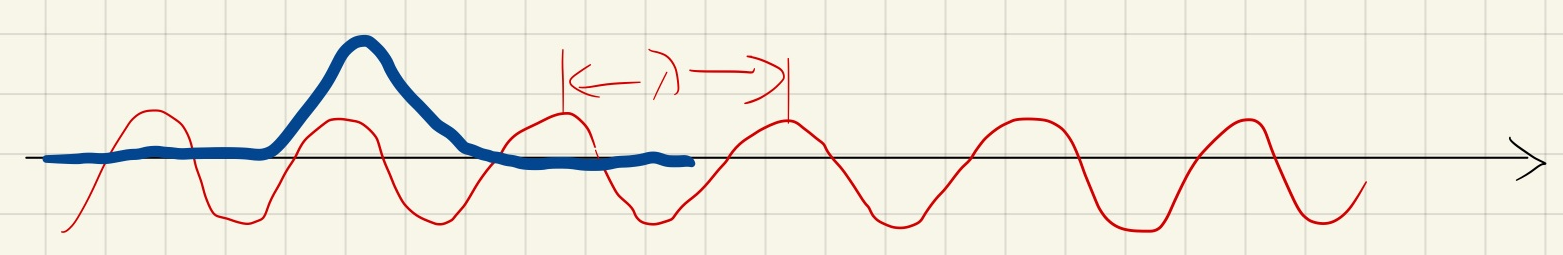
\includegraphics[width=1.0\textwidth]{fig/fig1-1.png}
  \caption{The example of wave with will and ill defined wavelength.}
  \label{fig:1-1}
\end{figure}

%%% Local Variables:
%%% mode: latex
%%% TeX-master: "main"
%%% End:
